\documentclass[prd,floatfix,preprintnumbers,amsmath,amssymb,nofootinbib,superscriptaddress]{revtex4}
\usepackage{graphicx}% Include figure filesg
\usepackage{subfigure}

\def\pheq{\phantom{=}}
\newcommand{\Deqn}[1]{{Eq.~(\ref{#1})}}
\newcommand{\Deqns}[1]{{Eqs.~(\ref{#1})}}
\newcommand{\Ceqn}[1]{{Equation~(\ref{#1})}}
\newcommand{\Dfig}[1]{{Fig.~\ref{#1}}}
\newcommand{\beq}{\begin{equation}}
\newcommand{\eeq}{\end{equation}}
\newcommand{\bea}{\begin{eqnarray}}
\newcommand{\eea}{\end{eqnarray}}
\newcommand{\tr}{{\mathop{\mathrm{tr}}\nolimits}}

\begin{document}


\title{Practicum 1}

\maketitle

\section*{Part A: Antenna Pattern Functions}

For this exercise you will be plotting antenna pattern functions for a pulsar-Earth system, and LIGO. 
You have a script that plots a sphere in 3d, and it needs to be modified to plot surfaces of different shapes.


\begin{itemize}

\item Use Eq. (7) of Ref.~\cite{Anholm} to plot the antenna pattern function for the plus-polarized gravitational wave, 
i.e. the geometrical pre-factor of the first term of the right hand side. If you don't know what a 
direction cosine is, wikipedia has a nice entry. Plot the cross-polarization antenna pattern. What is the difference?

\item Plot the antenna pattern response for LIGO using Eq. (3) of Ref.~\cite{Kazu}. Notice the antenna pattern 
function for LIGO has the polarization angle in it.  Plot it for a few different polarization angles. In the 
pulsar-Earth system used to derive Eq. (7) of Ref.~\cite{Anholm}, no polarization angle appears. 
What angle is degenerate with the polarization angle? (It may help to look at Figure 2 of Ref.~\cite{Kazu}.)

\begin{figure}
\centering
\mbox{\subfigure{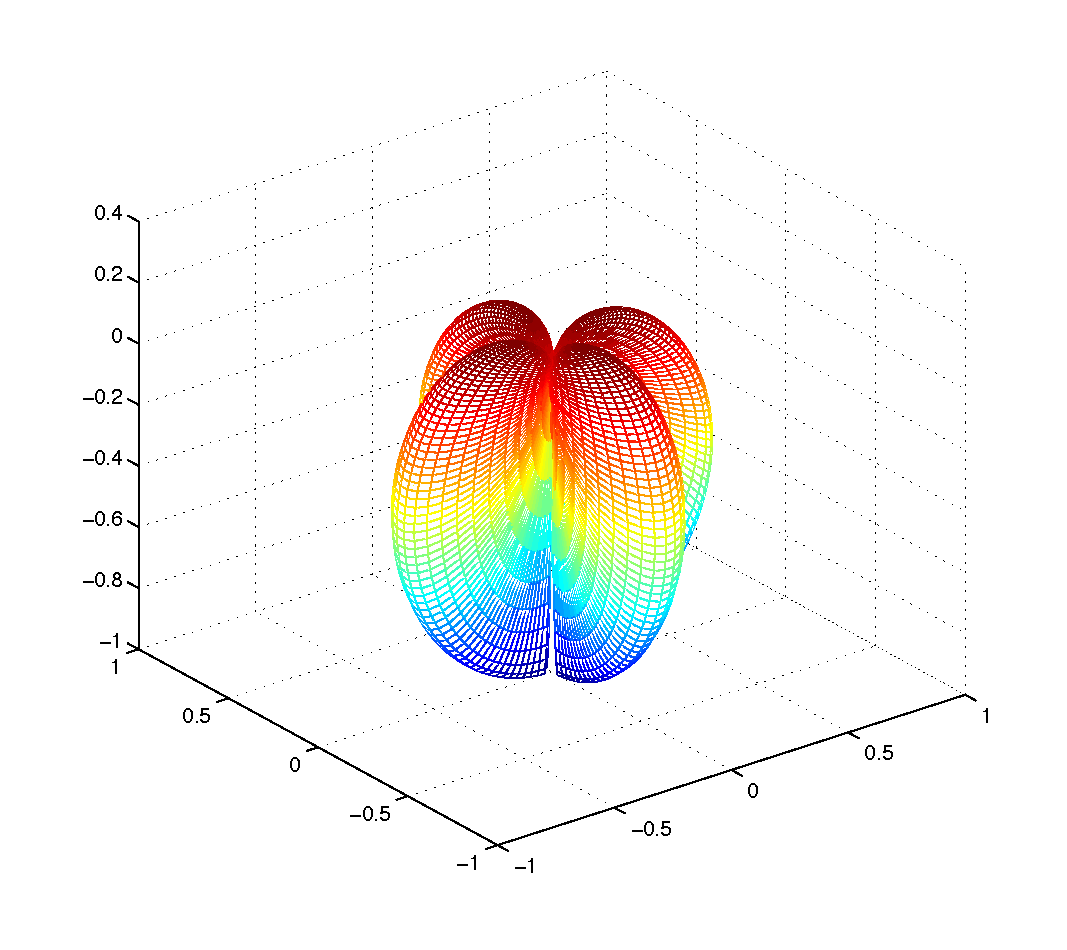
\includegraphics[width=8cm]{AntPulsar}}\quad
\subfigure{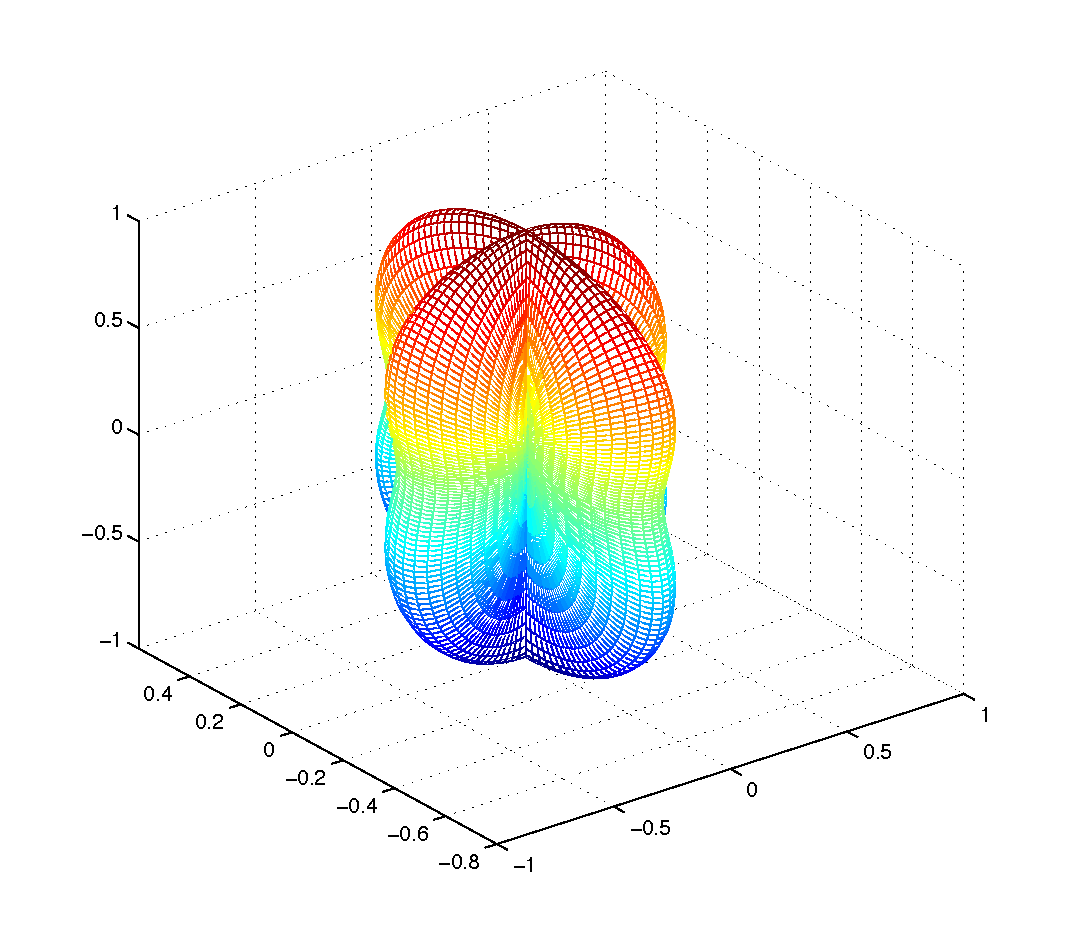
\includegraphics[width=8cm]{AntLIGO} }}
\caption{Antenna pattern foor the pulsar-Earth system (for plus-polarized waves) using Eq. (7) of Ref.~\cite{Anholm},
and antenna pattern for LIGO using Eq. (3) of Ref.~\cite{Kazu} with the polarization angle $\psi=0$.
} 
\end{figure}



\item Plot the frequency dependent antenna pattern response in Eq. (16) of \cite{Anholm}.  All you need to do 
is multiply what you used for the exercise in the first bullet point by the phase factor in the brackets in Eq. (16).  
Plot it for $fL=1$ and $fL=10$.  What are the differences? 

\begin{figure}
\centering
\mbox{\subfigure{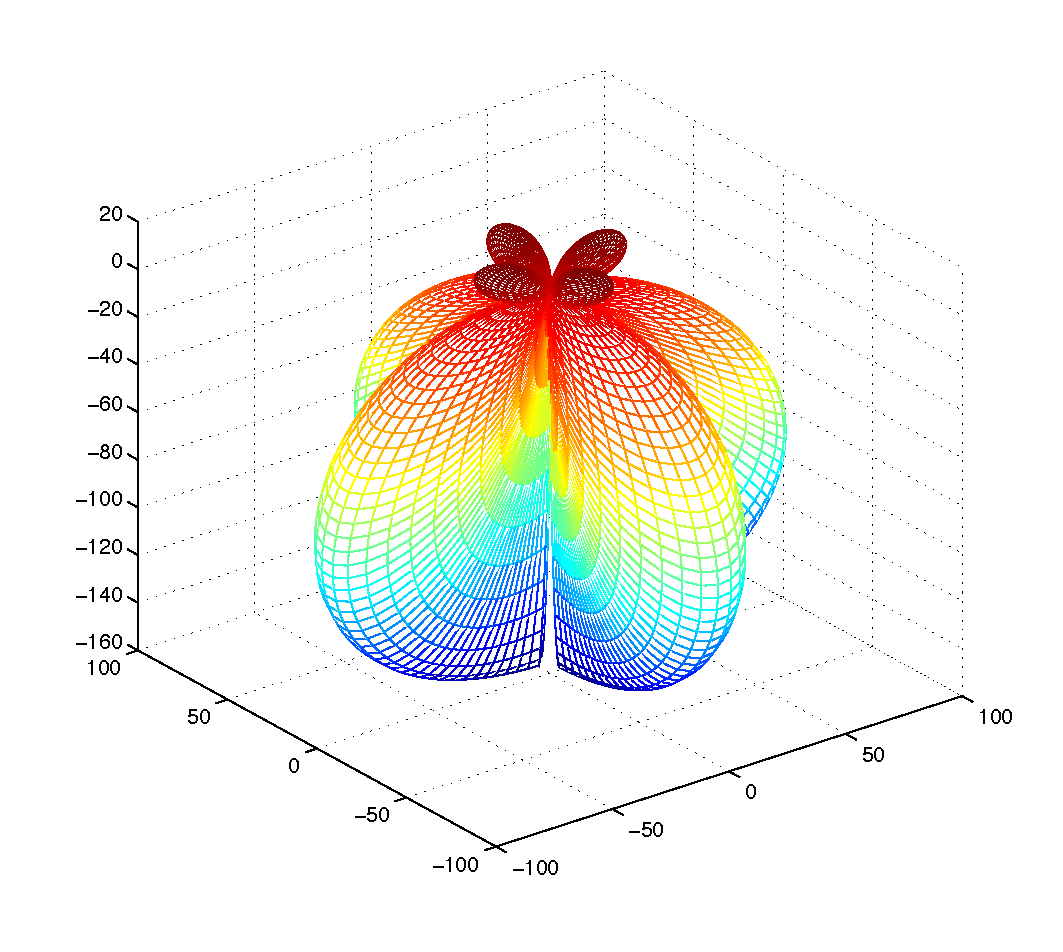
\includegraphics[width=8cm]{AntfL1}}\quad
\subfigure{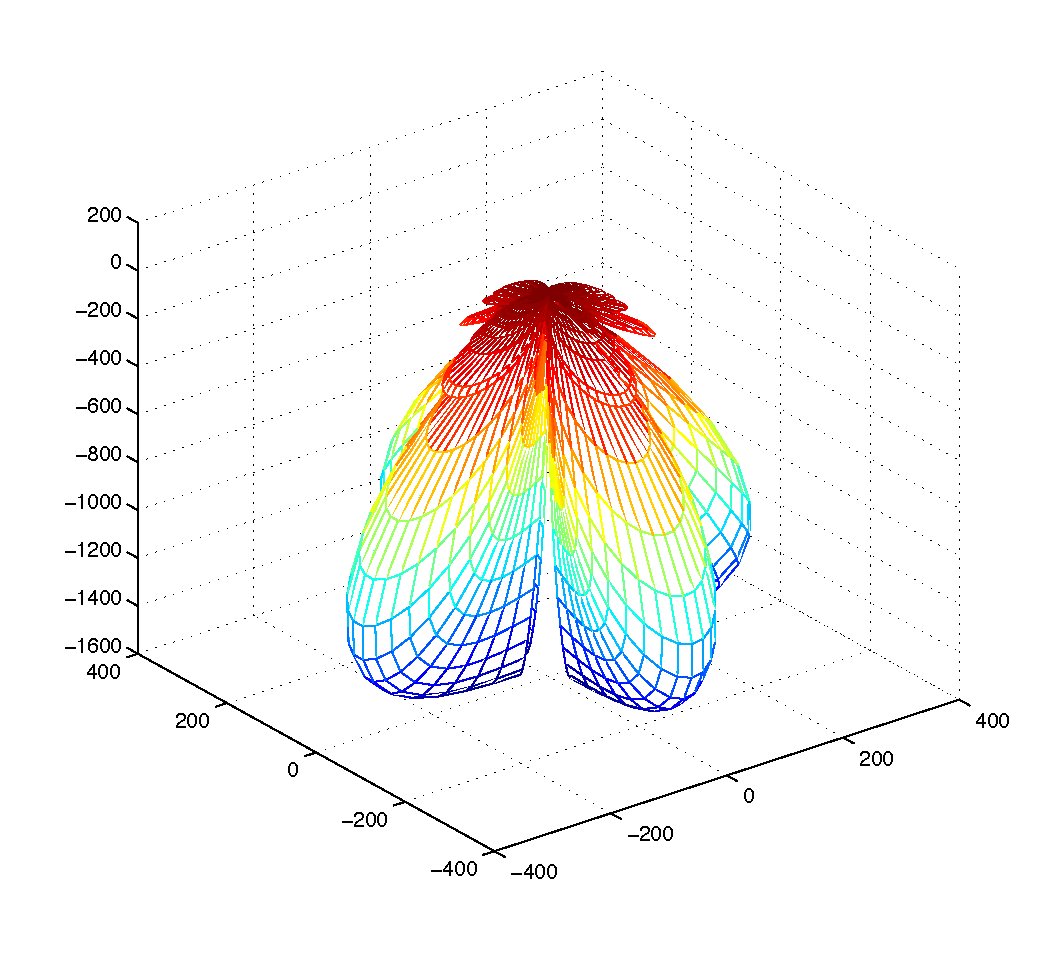
\includegraphics[width=8cm]{AntfL10} }}
\caption{Frequency domain antenna pattern that uses the phase factor Eq. (16) of Ref.~\cite{Anholm} for $fL=1$ and $fL=10$.} 
\end{figure}

\item The response appears to be singular when $\theta=\pi$.  Do a Taylor expansion of the frequency dependent
antenna pattern function, taking $\theta=\pi+\delta$, where $\delta$ is sufficiently small that the exponential 
can be expanded. Show that the response is not singular, proportional to $fL$, and in terms of this result, 
explain the differences you saw between $fL=1$ and $fL=10$ 
in the previous exercise. As a sidenote, it is worth pointing out that the extra sensitivity of the pulsar-Earth system
to longitudinal polarization modes (in non-GR theories of gravity) comes from this limit. 



\end{itemize}


\pagebreak

\section*{Part B: The stochastic background produced by SMBBH mergers}

This one is a little more advanced. In the following exercise you will learn how to 
make order of magnitude estimates of the stochastic background produced by a large number of incoherently 
superimposed individual gravitational wave sources. We will focus on the background
produced by the merger of supermassive black holes at the centers of galaxies.  I have given references
for most equations used, and included the papers as part of the materials. This excercise is 
self contained and you don't actually need to read the references, you can just go ahead and 
use the equations given. But if you're curious as to 
where the equations are coming from you can also go look them up.

The strength of the stochastic background as a function of frequency can be expressed in terms of 
the spectrum $\Omega_{\rm gw}(f)$ as follows
\beq
 \Omega_{\rm gw}(f)\equiv \frac{1}{\rho_{\rm crit}}\frac{d\rho_{\rm gw}}{d\ln f},
\label{omdef}
\eeq
where $\rho_{\rm crit}=8\pi/3H_0^2$ is the closure energy density of the Universe, $H_0$ 
is the current value of the Hubble parameter, and $\rho_{\rm gw}$ is the energy 
density in gravitational waves.  The strength of the background is often expressed in terms
of the characteristic strain, is sometimes written in terms of the characteristic strain
\beq
h_c^2(f)=\frac{3H_0^2}{2\pi^2}\frac{1}{f^2}\Omega_{\rm gw}(|f|).
\eeq


The background produced by all supermassive binary black hole coalescences in the Universe 
can be expressed as
\begin{equation}
\Omega_{\rm gw}(f) = \frac{4 \pi^2}{3H^2_0}f^3 
\int dz \int d\log M \, h^2(f,z,M)  \frac {d^2R}{dzd\log M},
\label{e:Omega(f)2}
\end{equation}
where $h(f,z,M)$ is the strain produced at frequency $f$, by a source of 
mass $M$ at redshift $z$, and $d^2R/dzd\log M$ is 
the rate of such events per unit redshift per unit logarithmic mass. NOTE: All logarithms here are base 10!
As I mentioned earlier, you do not need to understand where this comes from to complete this exercise 
but if you want to see a derivation of this result check out Section F and the discussion 
leading up to Eq. (56) of~\cite{Leblond} (this paper is about cosmic strings but you can just replace the 
string length $l$ with the mass $M$ above and the derivation is the same). This result is quite general.

Alberto Sesana has kindly provided an order of magnitude estimate for the SMBBH merger rate,
\beq
 \frac {d^2R}{dzd\log M} \sim C z^3 \left(\frac{M}{M_*}\right)^{0.7} e^{-(M/M_*)^{1/2}},
\eeq
where $M_*=10^{7.2} M_{\odot}$, which is valid only for $z<2$ and $M>10^7 M_{\odot}$, and $C$ is such that,
\beq
 \int_0^2 dz \int_7 ^\infty d\log M  \frac {d^2R}{dzd\log M}= 3 \times 10^{-2} {\rm yr}^{-1}.
\eeq
Remember all logarithms are base 10 here (see the mass integration limits).

The strain as a function opf frequency produced by a binary inspiral is~\cite{Thorne}
\beq
h(f,z,M) \sim g \sqrt{\frac{\pi}{12}} \frac{\mu}{r(z)} \frac{M_T^{3/2}}{\mu^{1/2}}
\frac{1}{(\pi M_T f)^{7/6}}(1+z)^{-1/6}, 
\eeq
where,
\beq
g=\left(\frac{G}{c^2}\right)^{5/6} c^{1/6} 
\eeq
is the factor needed to go from the geometrical units that Kip Thorne uses to physical units, 
$z$ is the redshift, $r(z)$ is the proper distance as a function of the redshift, 
$\mu=M_1 M_2/M_T$ is the reduced mass of the system, and $M_T$ is the total mass. 
Since this is an order of magnitude estimate, for simplicity you can take 
$M_1=M_2=M$. This is Eq. 44 of reference~\cite{Thorne}, 
an orientation averaged frequency domain waveform for binary inspirals in the Newtonian 
regime.  The only modifications I've made are including the effects of the redshift, and 
adding the conversion from geometrical to physical units.

Your task is to write a short piece of code that computes the characteristic strain as a 
function of frequency using the equations above. You have a short code with all the 
constants defined, and also an expression for $r(z)$. So you need to write the code 
for the integral, then load up the file 
pta\_2020.dat (kindly provided by Paul Demorest), and plot everything together.

\begin{figure}[h]
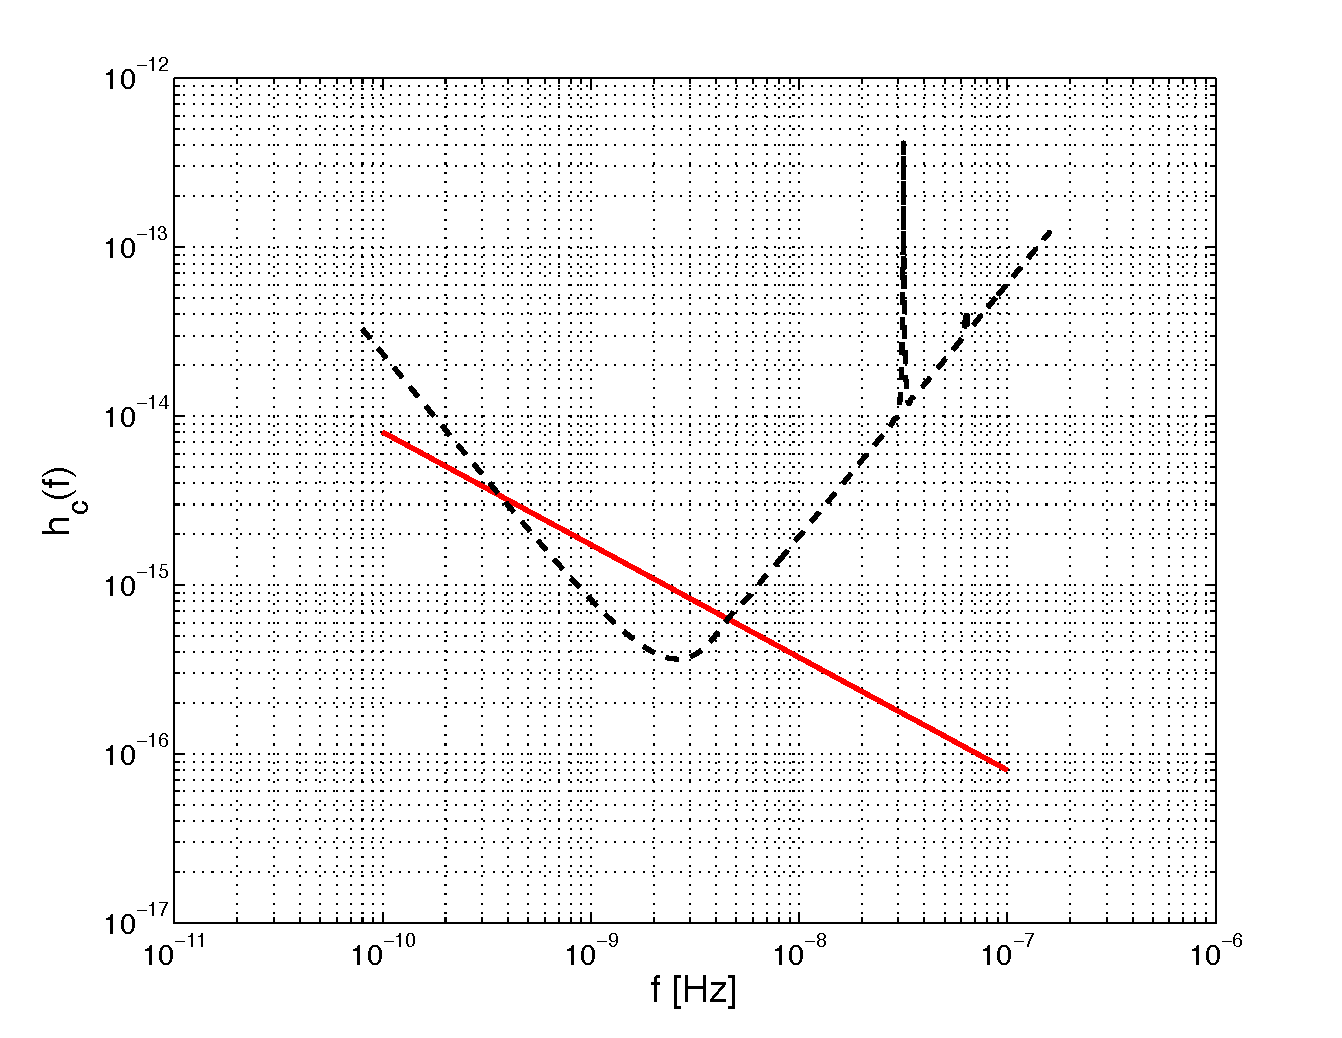
\includegraphics[width=11cm]{SMBBH}\\
\caption{Supermassive binary black hole stochastic background (red), and expected sensitivity (dashed black), expressed in terms of the
characteristic strain $h_c(f)$ versus frequency in Hz computed using the equations above.}
\end{figure}


\begin{thebibliography}{}

\bibitem{Anholm} Anholm et al.; Phys. Rev. D 79, 084030 (2009).

\bibitem{Kazu} Hayama et al. ; Phys. Rev. D 79, 082002 (2009).

\bibitem{Leblond} Leblond et al. ; Phys. Rev. D 79, 123519 (2009).
   
\bibitem{Thorne} K.S. Thorne in 300 years of gravitation. pp 380 (1987).

\end{thebibliography}
\end{document}
